% author: Jonah Miller
% inspired by Christian Feuersaenger

\documentclass[border=10pt]{standalone}
\usepackage{pgfplots}
%\pgfplotsset{width=7cm,compat=1.8}

\newcommand\expr[2]{exp(-#1^2) * sin(deg(#2))}

\begin{document}
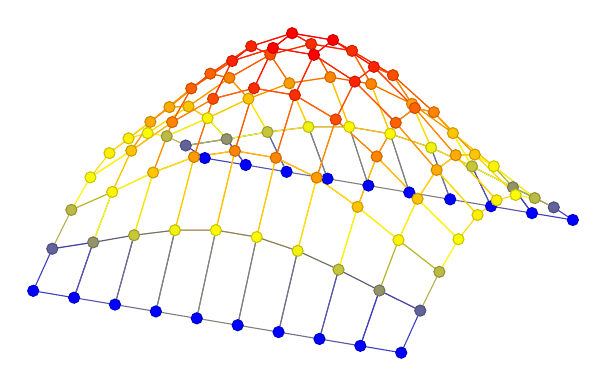
\begin{tikzpicture}
	\begin{axis}[
          grid=none,
          hide axis,
          domain=-1:1,
          domain y=0:pi,
          ]
	\addplot3[
        mesh,scatter,
        samples=10,
        shader=faceted interp,
        ] 
		{\expr{x}{y}};
	\end{axis}
\end{tikzpicture}
\end{document}